\section{Comparisons with UVIS occultations and GCMs predictions}

The extinction profiles retrieved in the previous sections can be compared with results
obtained with other instruments and Global Circulation Models (GCM) predictions.
\cite{West2018} already confirmed the excellent agreement between the observations made during
two Voyager flybys and the position of the detached haze layer one Titan year later.
Comparisons with VIMS and CIRS instruments, also onboard Cassini, could be possible but
they are limited by the sensitivity of their detectors above 450 km where the detached haze is located.
Therefore, we were only able to perform a comparison two stellar occultations
made by the UVIS instrument in 2009 \citep{Koskinen2011}.

\subsection{Comparison with UVIS occultations}

\cite{Koskinen2011} derived information on the mesosphere and thermosphere of Titan using UVIS stellar
occultations. The sensitivity to haze opacity of UVIS during a stellar occultation is much better than what ISS can achieve. However,
while ISS probes the light scattered by the detached haze layer, UVIS probes the light transmitted through a tangential
path at the limb. In both cases, an extinction profile can be retrieved. ISS can retrieve the extinction of the
particles which scatter light, and under assumptions concerning the phase function and the single scattering albedo \change{\citep{Seignovert2017, West2018}}.
On the other hand, UVIS is able to retrieve the total extinction from transmission with no assumption about the haze
particles. This difference is valuable because it may give information about the change in aerosol
size with altitude. In practice, ISS sensitivity is not sufficiently sensitive to probe above
the peak of the detached haze by more than a scale height.

Two of the UVIS occultation profiles, in 2008 and 2009 (T41 and T53 flybys), can be directly compared with ISS
observations at the same location and at the same period (Fig.~\ref{fig:uvis_iss}). The UVIS profiles are scaled to
offset the spectral dependence between ISS and UVIS effective wavelengths (338 nm and 1850-1900~\AA~respectively).
This offset is due to the spectral dependence of the extinction cross-sections and to the intrinsic
differences arising from comparing the extinction retrieved from scattering properties or from occultation
\citep[see.][]{Cours2011}.

\begin{figure}[!ht]
\plotone{Fig/UVIS_ISS}
\caption{Comparisons between ISS and UVIS extinction profiles before the equinox.
UVIS profiles are retrieved by \cite{Koskinen2011} during the T41 (2008/02/23) and T53 (2009/04/19) flybys.
ISS profiles are retrieved for the images N1585329510\_1 (2008/03/27) and
N1618568958\_1 (2009/04/16).
The UVIS profiles are scaled by a factor 0.15 to compensate the spectral dependence of the extinction
cross section and overlap ISS retrievals.}
\label{fig:uvis_iss}
\end{figure}

\change{The two profile can be compare in the 450 to 550 km altitude range.
In the first case (Fig.~\ref{fig:uvis_iss}a), even if the profiles don't exactly overlaps, the ISS extinction profile presents a peak of extinction exactly at the same location as the one observed by UVIS. The drop, above and below the peak is more pronounced with ISS than with UVIS.
In the second case (Fig.~\ref{fig:uvis_iss}b), the two profiles presents a excellent agreement with each over in the 450 to 550 km altitude range.}

Considering that UVIS and ISS profiles are not taken simultaneously and
they don't probe the same longitude, the results of the previous section demonstrate that these differences are
consistent with the natural variabilities observed in the detached haze layer.
This comparison is then a good validation of our results concerning the extinction profiles of the detached haze.

Above 575 km, UVIS extinction profiles show the presence of a secondary layer at 610 km which is not detected
by ISS. As shown by \cite{Cours2011}, ISS is only sensitive to the larger aerosols, those that scatter light, whereas
UVIS is able to probe the extinction of all the particles, and especially the smaller ones which do not scatter.
In theory, the difference between UVIS and ISS above 575 km may reveal a sharp change in aerosol size distribution.
But, this layer is located at altitudes where the signal to noise is low and \change{our model is no longer able to retrieve the extinction above this altitude.}
Therefore, it is not possible to draw a safe conclusion from the ISS profiles above 575 km.

\subsection{Comparison with general circulation models predictions}

General circulation models are very powerful tools to understand the climate of planetary atmospheres and the
interplay between different processes at planetary scale. In the case of Titan, circulation and haze are linked
by a strong feedback loop. The large scale structures in the haze layer are produced by the action of the
circulation. The haze layer produces a feedback effect on the circulation through the control of the stratospheric
thermal structure \citep{Rannou2004}. The detached haze is one of the noticeable feature produced by the the
stratospheric circulation \citep{Rannou2002, Lebonnois2012, Larson2015}. The figure.~\ref{fig:gcm_winter}
and \ref{fig:gcm_spring} show the maps of haze extinction obtained by \cite{Lebonnois2012} and
\cite{Larson2015} at 700 nm and 525 nm respectively. They can be compared with the extinction map derived
with ISS in the CL1-UV3 filters at 338 nm.

\begin{figure}[!ht]
    \centering
    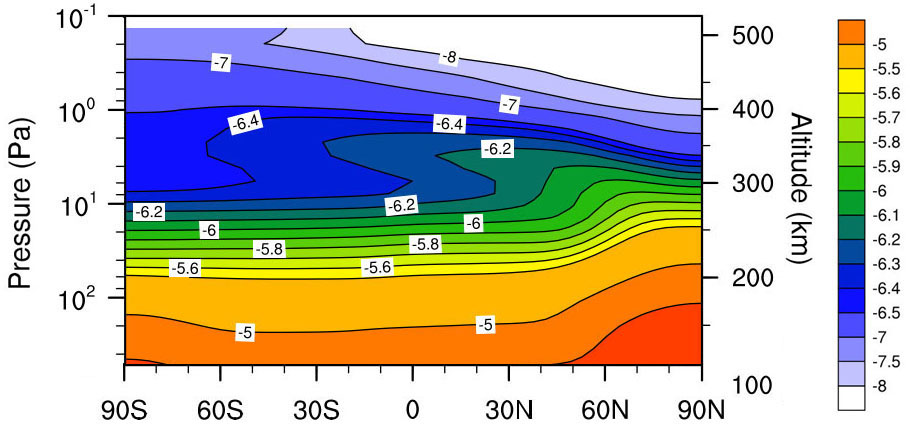
\includegraphics[width=.4\textwidth]{Fig/Lebonnois2012_Fig4_winter.jpg}
    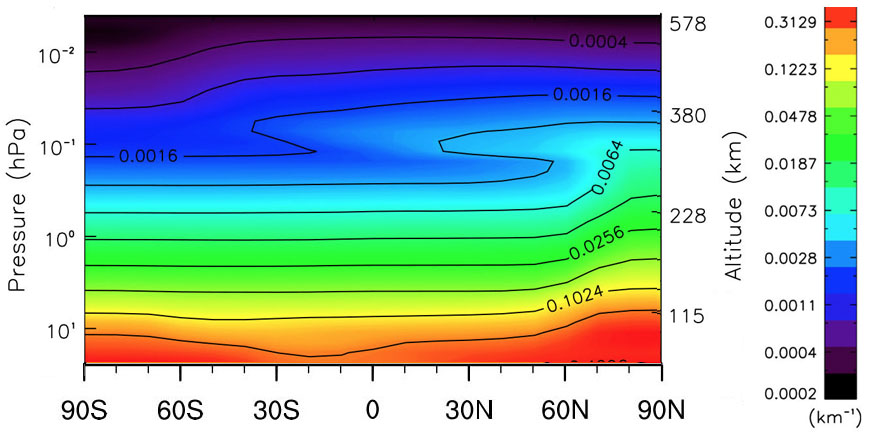
\includegraphics[width=.4\textwidth]{Fig/Larson2015-Fig7_Winter.jpg}
    \includegraphics[width=.8\textwidth]{Fig/N1477222048_2-lat_beta.png}
    \caption{At the top, the zonally averaged haze extinction at the northern winter solstice
        ($L_s = \ang{270}$) estimated by \cite{Lebonnois2012} at the wavelength $\lambda = $ 700 nm (left)
        and by \cite{Larson2015} at $\lambda = $ 525 nm (right). At the bottom, haze extinction map
        retrieved from Cassini/ISS observation CL1-UV3 ($\lambda = $ 338 nm) in the middle of the winter
        (\textbf{N1477222048\_2} - $L_s = \ang{300}$).}
    \label{fig:gcm_winter}
\end{figure}

At the northern winter solstice (Fig.~\ref{fig:gcm_winter}), the detached haze appears around 350 km
in both models. In \cite{Lebonnois2012}, the altitude decreases by about few tens of km from the southern latitudes to
the north polar region where it merges with the north polar hood at ($\simeq$ \ang{40}N). In \cite{Larson2015}, the detached
haze remains at constant altitude, appears better marked than in \cite{Lebonnois2012}, and merge with the polarhood
around \ang{60}N. In both models, the extinction increases from the south to the north by about a half magnitude.
In the observations made in 2004, \emph{i.e.} at the middle of the winter, the detached haze layer is completely developed at
500 km and covers latitudes from the south polar region to \ang{60}N where it merges with the north polarhood. The
location of the depletion zone decreases from 475 to 425 km between \ang{40}N and \ang{60}N, which is not the case in
models. It is, on the other hand, consistent with the results obtain from stellar occultation by \cite{Sicardy2006}.
The haze extinction increases from the south to the north with about the same magnitude than in models. This
is consistent with a layer increasing in aerosol loading while the airmass is flowing from south to north. It was already
noted \citep{West2011, West2018} that the detached haze layer in models appears as a supplementary layer added to
the background aerosols while, in data, it appears detached because there is an intermediated zone strongly depleted in
aerosols. Finally, as mentioned before, the detached haze layer is continuous all around the South Pole, which is not
the case in the models.

\begin{figure}[!ht]
    \centering
    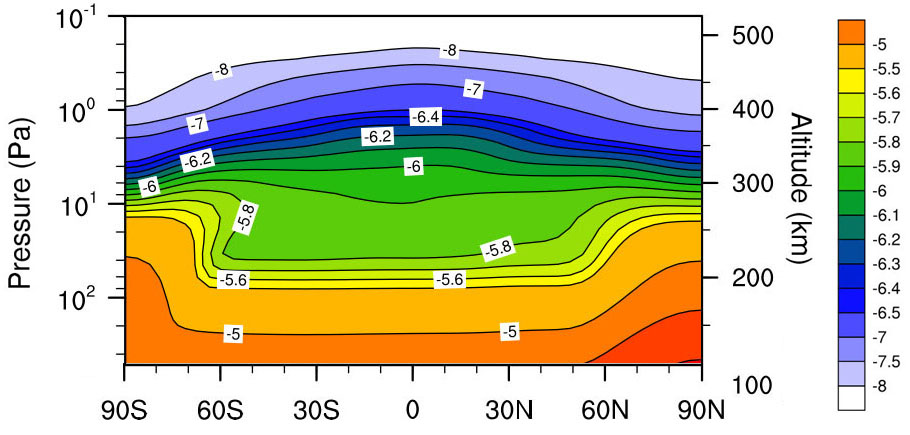
\includegraphics[width=.4\textwidth]{Fig/Lebonnois2012_Fig4_equinox.jpg}
    \includegraphics[width=.4\textwidth]{Fig/Larson2015-Fig7_Spring.jpg}
    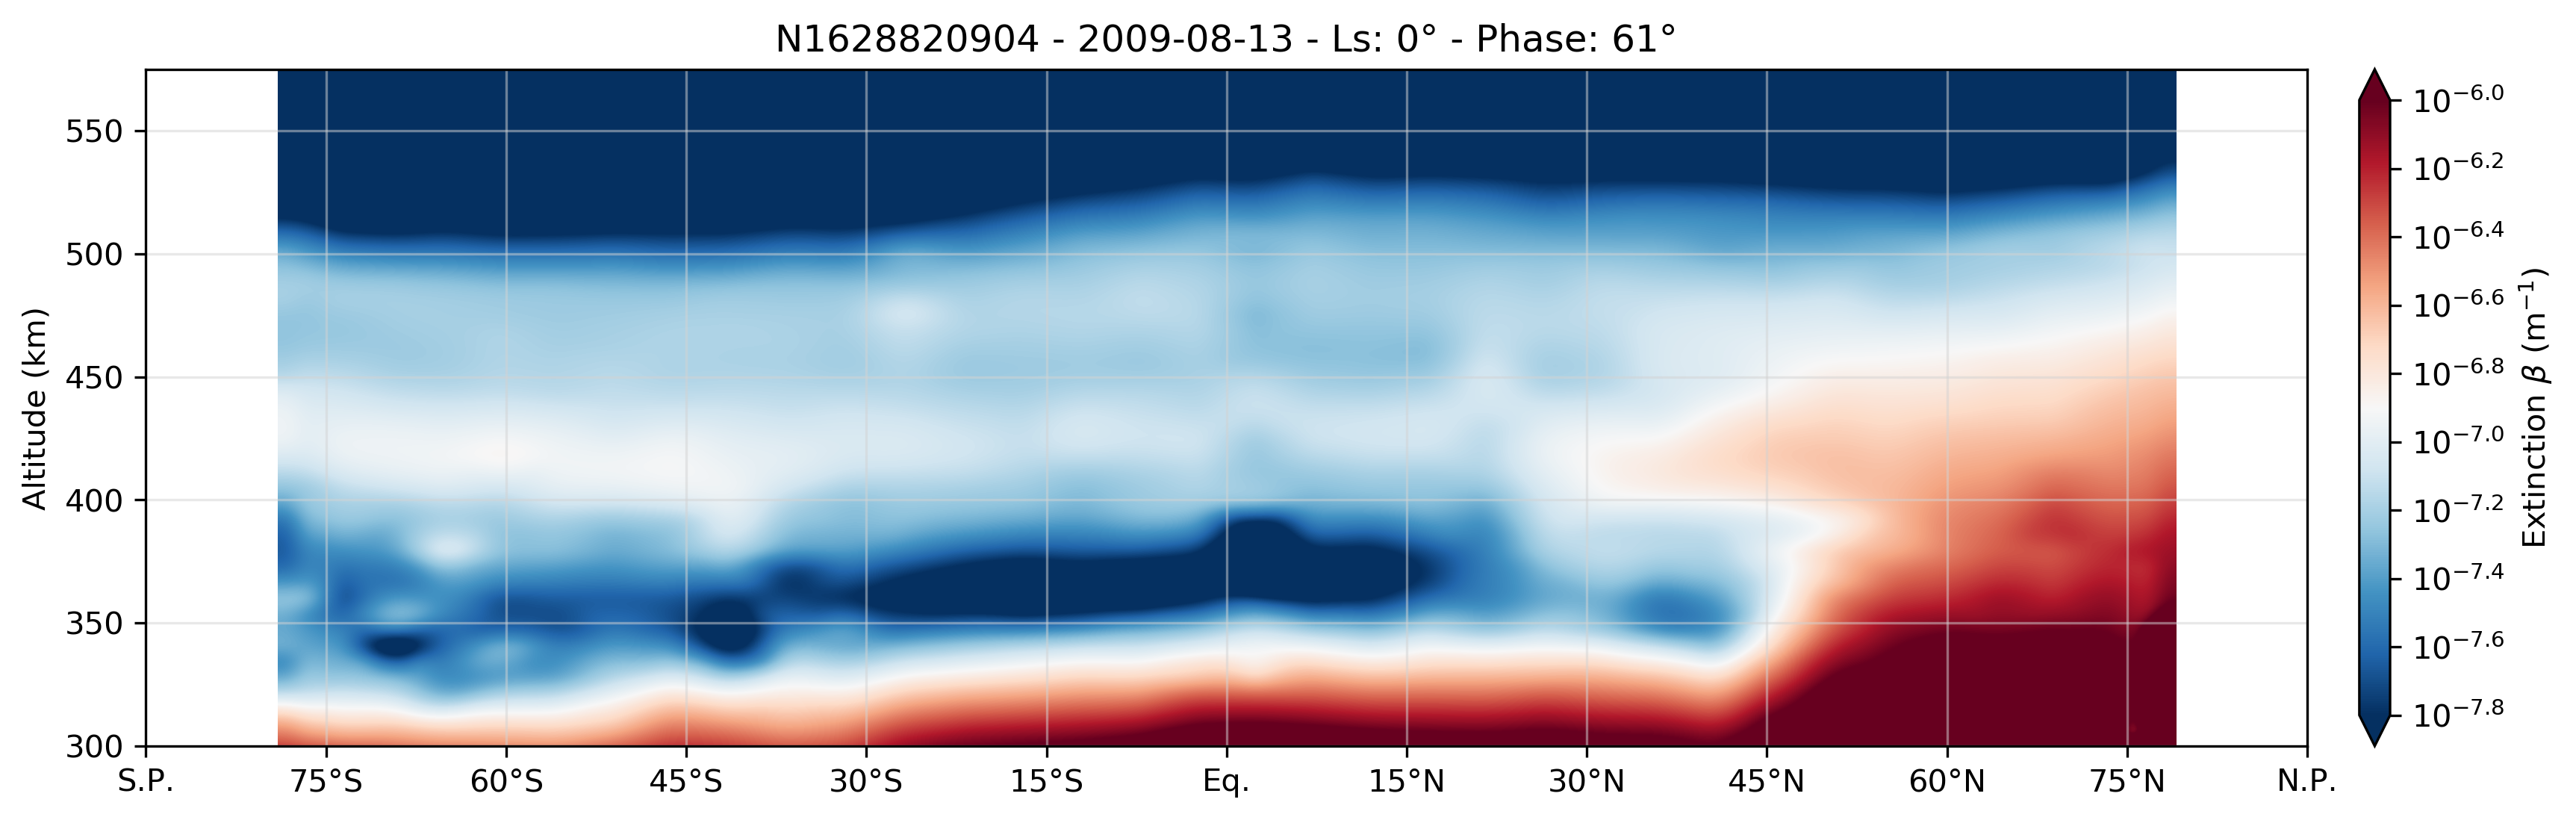
\includegraphics[width=.8\textwidth]{Fig/N1628820904_1-lat_beta.png}
    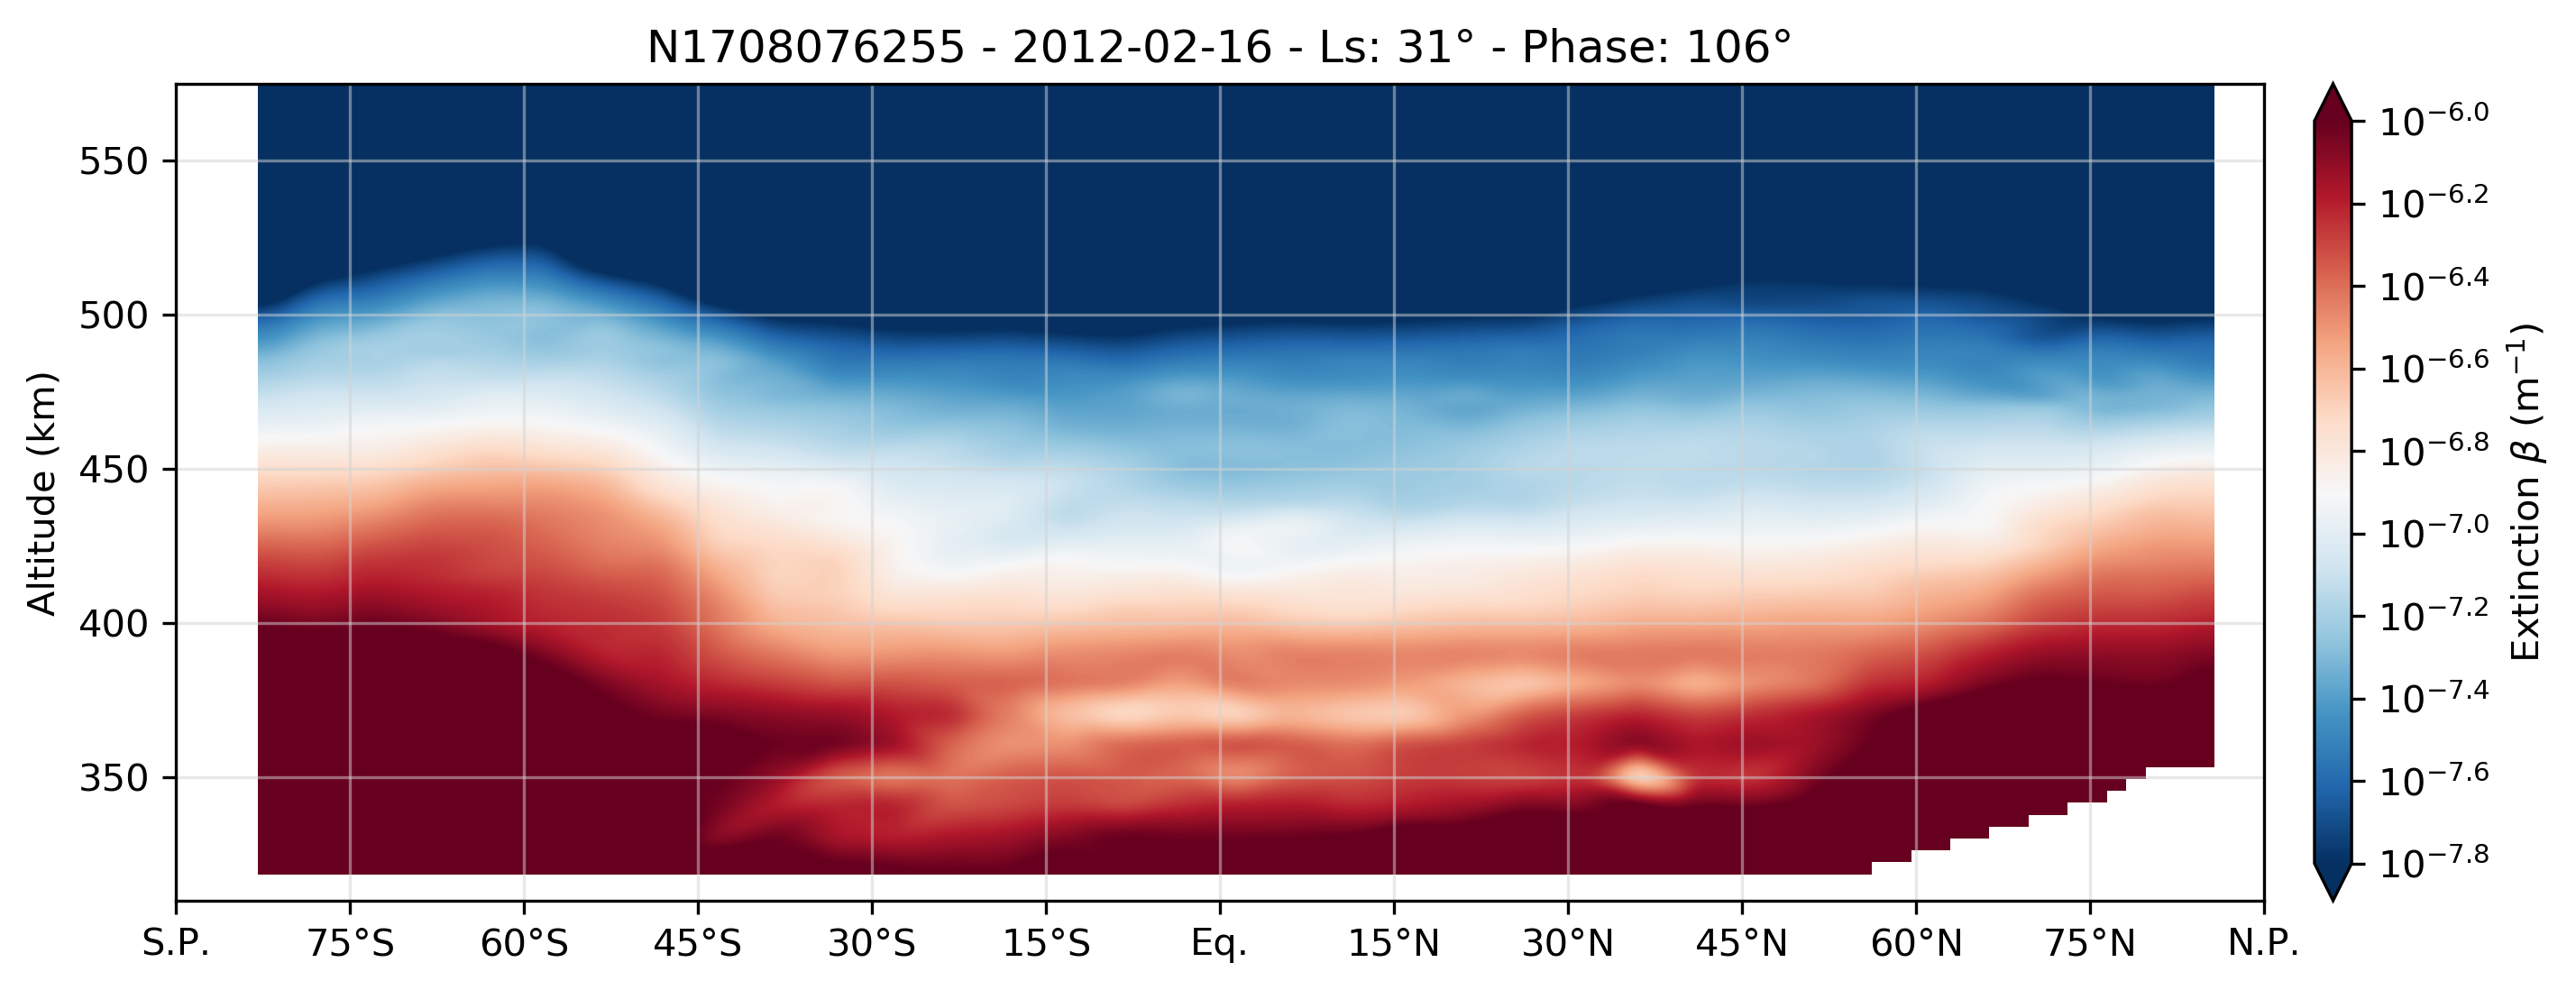
\includegraphics[width=.8\textwidth]{Fig/N1708076255_1-lat_beta.png}
    \caption{At the top, the zonally averaged haze extinction at the northern spring equinox ($L_s = \ang{3}$)
        estimated by \cite{Lebonnois2012} (left) and at 1000 days after the equinox ($L_s = \ang{30}$)
        by \cite{Larson2015} (right).
        At the bottom, two panels showing the haze extinction map retrieved from the Cassini/ISS observations
        at the Northern Spring equinox (\textbf{N1628820904\_1} - $L_s = \ang{0}$) and 1000 days after the equinox
        (\textbf{N1708076255\_1} - $L_s = \ang{30}$).}
    \label{fig:gcm_spring}
\end{figure}

At the northern spring equinox (Fig.~\ref{fig:gcm_spring}), the model from \cite{Lebonnois2012} shows a
flat main haze layer without detached haze between \ang{60}S and \ang{60}N and with two major increases at both poles. The
haze at south is increasing as a consequence of the circulation reversal while the northern haze is no more feeded
and will disappear later in the season. In observations (first panel of Fig.~\ref{fig:gcm_spring}),
this thicker haze is observed only for the northern latitudes, the detached haze has not yet disappeared and
and the feeding of the south polar haze has not started yet. To notice a major increase of extinction at the South Pole,
we need to wait until the beginning of the spring at $L_s = \ang{30}$ (second panel Fig.~\ref{fig:gcm_spring}).
At that period, the detached haze layer almost completely collapsed on the main haze and the haze distribution is very
similar to the one predicted by \cite{Lebonnois2012} at the equinox. In \cite{Larson2015}, 1000 days after the equinox,
we also observed a \emph{U} shape in the haze extinction as in data, but in this case, a new detached haze layer already
started to grow from the South Pole in the model whereas in data (second panel  of Fig.~\ref{fig:gcm_spring}) the local
increase seen at 380 km is the consequence of the drop of a previous secondary layer (cf. Figs.~\ref{fig:dhl_2008_2012}g
and \ref{fig:dhl_2008_2012}h). In both comparisons, this means that the timing in the circulation models is not in
phase with the reality. The model of \cite{Lebonnois2012} seems to be in advance by about 3 years compared to the data.
We have not enough information to characterize the advance in phase of \cite{Larson2015} model.

The timing and the scale of the drop predicted by both models (Fig.~\ref{fig:gcm_cycle}) globally match
the observations after the vernal equinox. The abrupt decrease of the vertical winds could be the cause of the fall of
the detached haze layer at the aerosol terminal speed. On the other hand, the timing and the scale of the reappearance
of the detached haze layer in models does not follow exactly the observations. Announced in late 2014 or early 2015
($L_s = \ang{60}$) by \cite{Larson2015} or in mid-2017 ($L_s = \ang{90}$) by \cite{Lebonnois2012}, the detached haze layer
finally reappeared in late 2015 to early 2016.
However, in May 2017, the upper atmosphere of Titan is still evolving and does not present a polar hood in the South Pole
similar to the one observed in 2004. Moreover, the most recent observations of mid-2017 seem to show that the seasonal
formation of the detached haze layer could be different from one hemisphere to the other. The double peaks at
420 and 450 km in the temperature gradient profile, a proxy for the haze extinction, obtained from the 1989
occultation \citep{Sicardy1999} supports this hypothesis.

\begin{figure}[!ht]
    \centering
    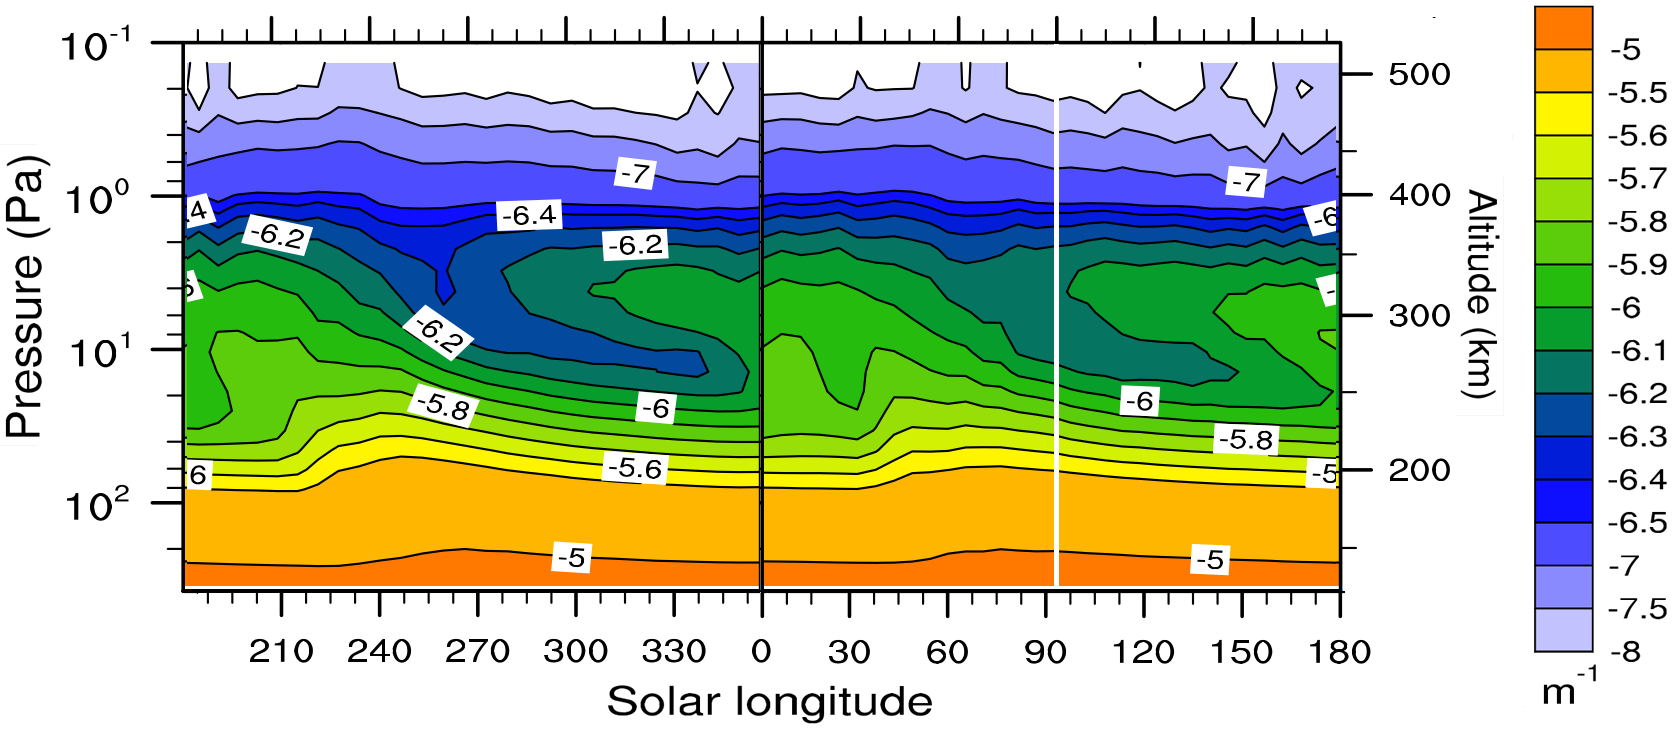
\includegraphics[width=.4\textwidth]{Fig/Lebonnois2012_dhl_cycle.png}
    \includegraphics[width=.4\textwidth]{Fig/Larson2015_dhl_cycle.png}
    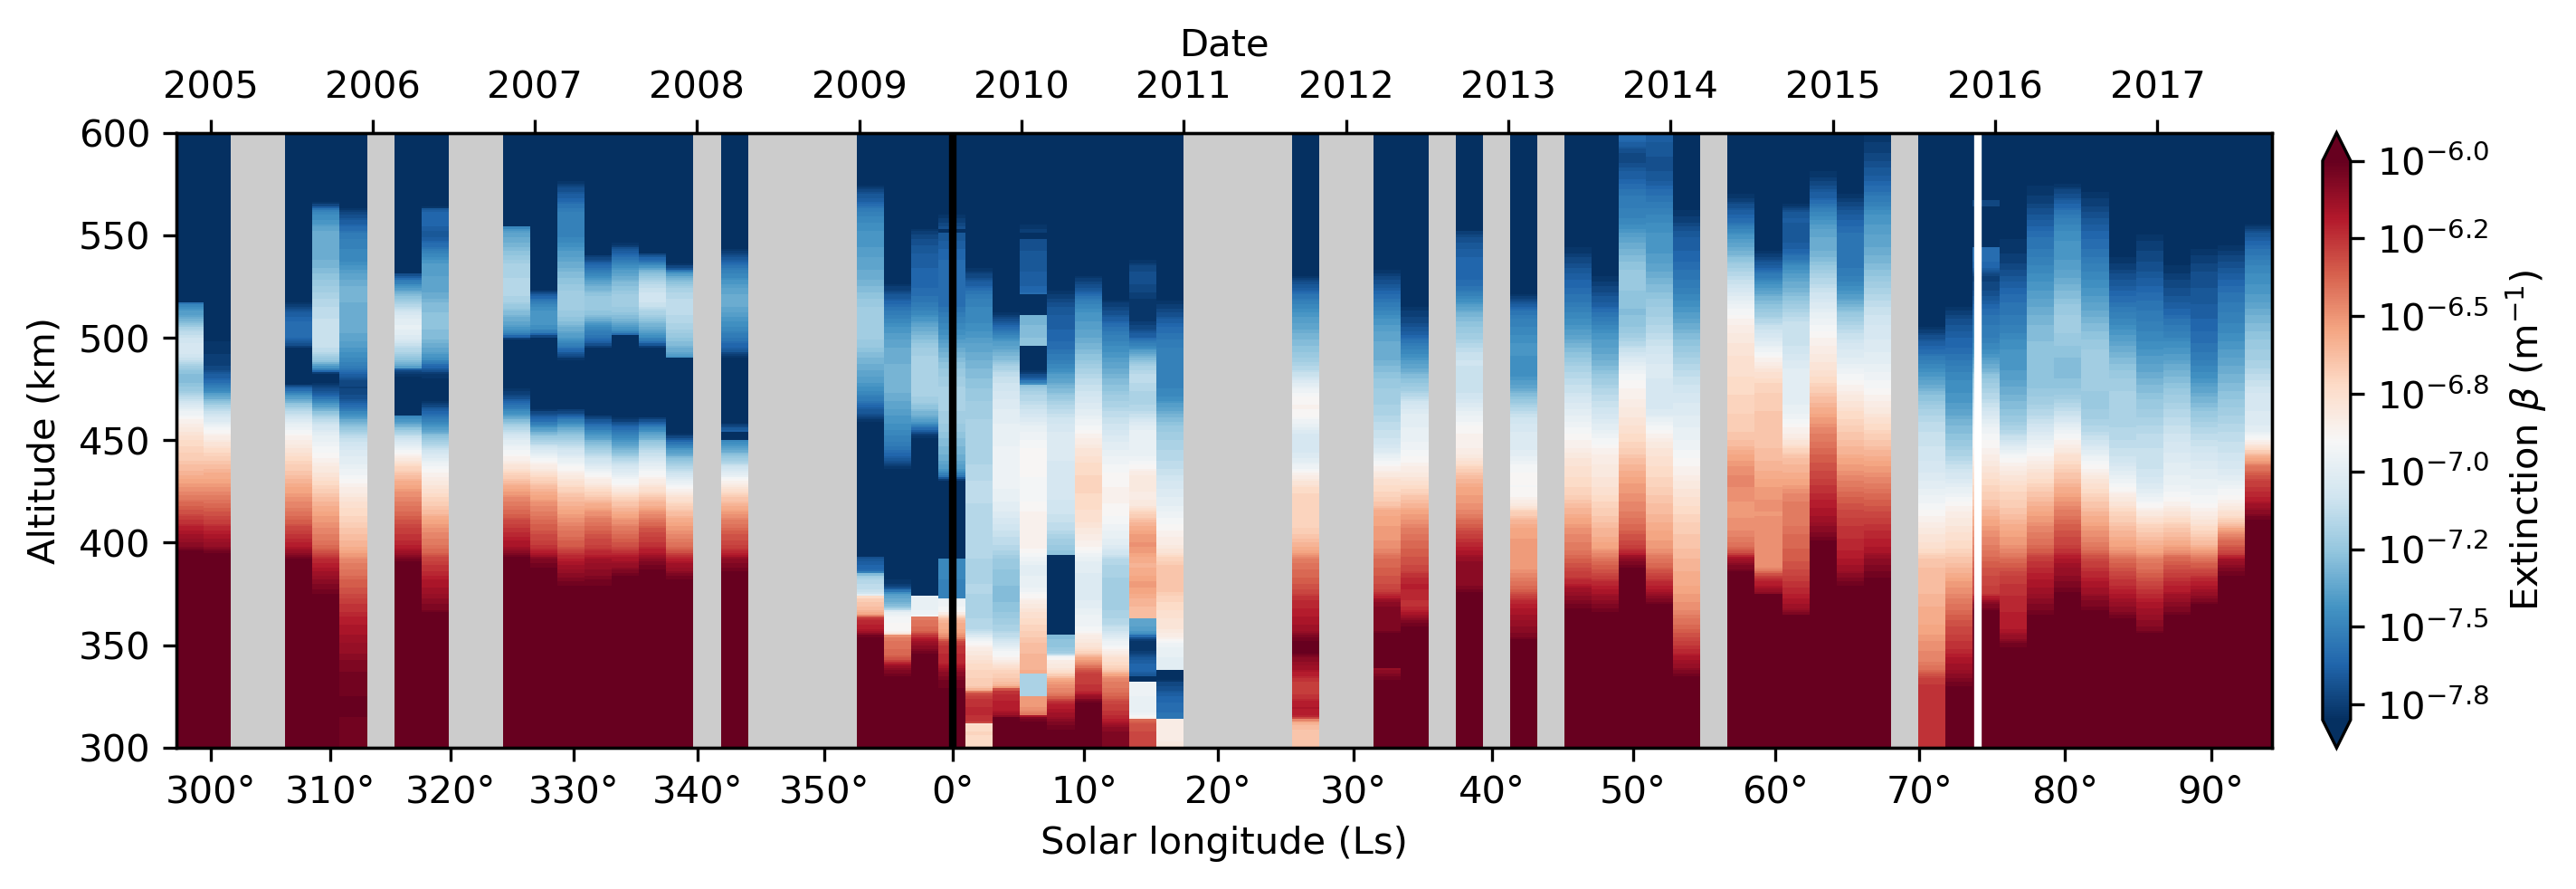
\includegraphics[width=.8\textwidth]{Fig/DHL_time_eq.jpg}
    \caption{Top-right: the annual variations of the zonally averaged equatorial opacity at 700 nm adapted
        from \cite{Lebonnois2012}.
        Top-left: the seasonal evolution of the aerosols mass density (g/cm$^3$) adapted from \cite{Larson2015}. The white dots are the local maximum of extinction extracted from the model.
        In both figures, the white vertical line correspond to the predicted date of the reappearance of the
        detached haze layer (after $L_s = \ang{90}$ and after $L_s = \ang{60}$ respectively).
        Bottom: the haze extinction as a function of time an altitude at the equatorial.
        % FIXME: Redo alt vs. time plot at Eq.
    }
    \label{fig:gcm_cycle}
\end{figure}

The current general circulation models do not match some of the large scale features reported before. The first of them
is the shape of the vertical extinction profile which has a local depletion, producing the detached haze layer, in the
observations while it simply appears as a high altitude haze layer superimposed to the main background haze in models.
The amplitude of the observed depletion reported, before and during the collapse, is sufficient to consider that the
detached haze layer is really disconnected from the main haze. We already stressed that the detached haze layer is
continuous around the South Pole without any visible upwelling coming from the main haze at this location. Finally, we
reported an early contraction of the main haze in 2008, just before the drop of the detached haze at the equinox. The origin
for such a contraction should be related with the weakening of the Hadley cell when the latitudinal illumination gradient
decreases around the equinox.

Thanks to high spatial resolution of the ISS NAC camera, we noticed some small scale structures which could be unresolved or
erased by the temporal averaging in GCMs. During the northern winter and spring, we observed some sporadic decreases and
bursts in the extinction profiles at very short time scale. These events could have a major impact on the redistribution of
aerosols in the upper atmosphere. We also reported in numerous cases, the existence of sub-layers above the main detached
haze with large latitude extend. Usually, their presence could be followed during more than an Earth year. This is
especially true during the collapse of the main detached haze layer after the equinox, when we observed several smaller
drops from 500 km down to 300 km. And finally, the double structure reported in 2016-2017
(Figs.~\ref{fig:dhl_2015_2017}c and \ref{fig:dhl_2015_2017}d) with two very distinct detached haze layers in the
North at 450 km, in the South at 520 km, was never mentioned before and needs a new interpretation.
